

\tikzset{every picture/.style={line width=0.75pt}} %set default line width to 0.75pt        

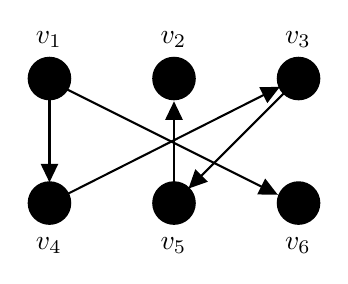
\begin{tikzpicture}[x=0.75pt,y=0.75pt,yscale=-1,xscale=1]
%uncomment if require: \path (0,144); %set diagram left start at 0, and has height of 144

%Straight Lines [id:da7193850870149698] 
\draw    (40,42) -- (40,88) ;
\draw [shift={(40,91)}, rotate = 270] [fill={rgb, 255:red, 0; green, 0; blue, 0 }  ][line width=0.08]  [draw opacity=0] (8.93,-4.29) -- (0,0) -- (8.93,4.29) -- cycle    ;
%Straight Lines [id:da1942442489782492] 
\draw    (40,42) -- (147.32,95.66) ;
\draw [shift={(150,97)}, rotate = 206.57] [fill={rgb, 255:red, 0; green, 0; blue, 0 }  ][line width=0.08]  [draw opacity=0] (8.93,-4.29) -- (0,0) -- (8.93,4.29) -- cycle    ;
%Straight Lines [id:da810447408180448] 
\draw    (100,92) -- (100,55) ;
\draw [shift={(100,52)}, rotate = 450] [fill={rgb, 255:red, 0; green, 0; blue, 0 }  ][line width=0.08]  [draw opacity=0] (8.93,-4.29) -- (0,0) -- (8.93,4.29) -- cycle    ;
%Straight Lines [id:da5553980379264378] 
\draw    (160,41) -- (109.12,91.88) ;
\draw [shift={(107,94)}, rotate = 315] [fill={rgb, 255:red, 0; green, 0; blue, 0 }  ][line width=0.08]  [draw opacity=0] (8.93,-4.29) -- (0,0) -- (8.93,4.29) -- cycle    ;
%Shape: Circle [id:dp8635781174027584] 
\draw  [color={rgb, 255:red, 0; green, 0; blue, 0 }  ,draw opacity=1 ][fill={rgb, 255:red, 0; green, 0; blue, 0 }  ,fill opacity=1 ] (30,41) .. controls (30,35.48) and (34.48,31) .. (40,31) .. controls (45.52,31) and (50,35.48) .. (50,41) .. controls (50,46.52) and (45.52,51) .. (40,51) .. controls (34.48,51) and (30,46.52) .. (30,41) -- cycle ;
%Shape: Circle [id:dp5046309407375] 
\draw  [color={rgb, 255:red, 0; green, 0; blue, 0 }  ,draw opacity=1 ][fill={rgb, 255:red, 0; green, 0; blue, 0 }  ,fill opacity=1 ] (90,41) .. controls (90,35.48) and (94.48,31) .. (100,31) .. controls (105.52,31) and (110,35.48) .. (110,41) .. controls (110,46.52) and (105.52,51) .. (100,51) .. controls (94.48,51) and (90,46.52) .. (90,41) -- cycle ;
%Shape: Circle [id:dp9523637573320518] 
\draw  [color={rgb, 255:red, 0; green, 0; blue, 0 }  ,draw opacity=1 ][fill={rgb, 255:red, 0; green, 0; blue, 0 }  ,fill opacity=1 ] (150,41) .. controls (150,35.48) and (154.48,31) .. (160,31) .. controls (165.52,31) and (170,35.48) .. (170,41) .. controls (170,46.52) and (165.52,51) .. (160,51) .. controls (154.48,51) and (150,46.52) .. (150,41) -- cycle ;
%Shape: Circle [id:dp46076804005955263] 
\draw  [color={rgb, 255:red, 0; green, 0; blue, 0 }  ,draw opacity=1 ][fill={rgb, 255:red, 0; green, 0; blue, 0 }  ,fill opacity=1 ] (30,101) .. controls (30,95.48) and (34.48,91) .. (40,91) .. controls (45.52,91) and (50,95.48) .. (50,101) .. controls (50,106.52) and (45.52,111) .. (40,111) .. controls (34.48,111) and (30,106.52) .. (30,101) -- cycle ;
%Shape: Circle [id:dp780817892587097] 
\draw  [color={rgb, 255:red, 0; green, 0; blue, 0 }  ,draw opacity=1 ][fill={rgb, 255:red, 0; green, 0; blue, 0 }  ,fill opacity=1 ] (90,101) .. controls (90,95.48) and (94.48,91) .. (100,91) .. controls (105.52,91) and (110,95.48) .. (110,101) .. controls (110,106.52) and (105.52,111) .. (100,111) .. controls (94.48,111) and (90,106.52) .. (90,101) -- cycle ;
%Shape: Circle [id:dp33231757908254456] 
\draw  [color={rgb, 255:red, 0; green, 0; blue, 0 }  ,draw opacity=1 ][fill={rgb, 255:red, 0; green, 0; blue, 0 }  ,fill opacity=1 ] (150,101) .. controls (150,95.48) and (154.48,91) .. (160,91) .. controls (165.52,91) and (170,95.48) .. (170,101) .. controls (170,106.52) and (165.52,111) .. (160,111) .. controls (154.48,111) and (150,106.52) .. (150,101) -- cycle ;
%Straight Lines [id:da4251496567702082] 
\draw    (40,101) -- (148.32,46.35) ;
\draw [shift={(151,45)}, rotate = 513.23] [fill={rgb, 255:red, 0; green, 0; blue, 0 }  ][line width=0.08]  [draw opacity=0] (8.93,-4.29) -- (0,0) -- (8.93,4.29) -- cycle    ;

% Text Node
\draw (32,17) node [anchor=north west][inner sep=0.75pt]    {$v_{1}$};
% Text Node
\draw (92,17) node [anchor=north west][inner sep=0.75pt]    {$v_{2}$};
% Text Node
\draw (152,17) node [anchor=north west][inner sep=0.75pt]    {$v_{3}$};
% Text Node
\draw (32,116) node [anchor=north west][inner sep=0.75pt]    {$v_{4}$};
% Text Node
\draw (92,116) node [anchor=north west][inner sep=0.75pt]    {$v_{5}$};
% Text Node
\draw (152,116) node [anchor=north west][inner sep=0.75pt]    {$v_{6}$};


\end{tikzpicture}